\documentclass[conference]{IEEEtran}
\usepackage[utf8]{inputenc}
\usepackage{graphicx}
\usepackage{amsmath}
\usepackage{url}
\usepackage{cite}

\title{Proyecto final análisis Exploratorio}

\author{
    \IEEEauthorblockN{Leopoldo Muñoz, Valentina Yáñez}
    \IEEEauthorblockA{
        Universidad de Talca \\
        Facultad de Ingeniería \\
        \texttt{leom18@alumnos.utalca.cl, vyanez20@alumnos.utalca.cl}
    }
}

\begin{document}

\maketitle

\begin{abstract}
This study explores the use of exploratory data analysis techniques and unsupervised clustering on a dataset of user sessions collected through Google Analytics. The influence of data points was analyzed using Cook's distance. The quality of the clusters was evaluated using the Hopkins statistic and the silhouette coefficient, applying algorithms such as K-Means, DBSCAN, Agglomerative Clustering, and GMM. The analysis revealed a tendency to form two clusters, enabling the exploration of differentiated strategies to improve conversion rates in e-commerce in the future.
\end{abstract}

\begin{IEEEkeywords}
Clustering, PCA, K-Means, E-commerce, Análisis Exploratorio de Datos, Hopkins, DBSCAN
\end{IEEEkeywords}

\section{Introducción}
El análisis del comportamiento de usuarios en plataformas de e-commerce es un pilar fundamental para la mejora de estrategias comerciales. En este trabajo se analiza un dataset con más de 12.000 sesiones de navegación anónimas, con el objetivo de agruparlas según patrones comunes mediante técnicas de clustering no supervisado.

\section{Descripción del Dataset}
El dataset fue obtenido del UCI Machine Learning Repository. Contiene 12.330 instancias (una por sesión) y 18 atributos (entre ellos, número de páginas vistas, duración de visitas, tasas de rebote, día de la semana, tipo de visitante, etc.). La variable objetivo Revenue fue eliminada para permitir un análisis no supervisado.

\section{Preprocesamiento de Datos}
No se encontraron valores faltantes. Las variables categóricas fueron convertidas a tipo \texttt{category} y procesadas con one-hot encoding. Las numéricas fueron escaladas. Se utilizó \texttt{RobustScaler} para atributos con alta influencia (como \texttt{BounceRates} y \texttt{SpecialDay}) y \texttt{StandardScaler} para el resto.


\section{Tendencia a Agrupamiento}
Se aplicó el estadístico de Hopkins, obteniéndose un valor de $0.9785$, lo que indica una fuerte tendencia a formar clusters.
\section{Reducción de Dimensionalidad}
Se utilizó Análisis de Componentes Principales (PCA), conservando que los primeros 5 componentes explican el más del 85\% de la varianza acumulada. Estas fueron usadas para visualizar los resultados de clustering.
\begin{figure}[htbp]
    \centering
    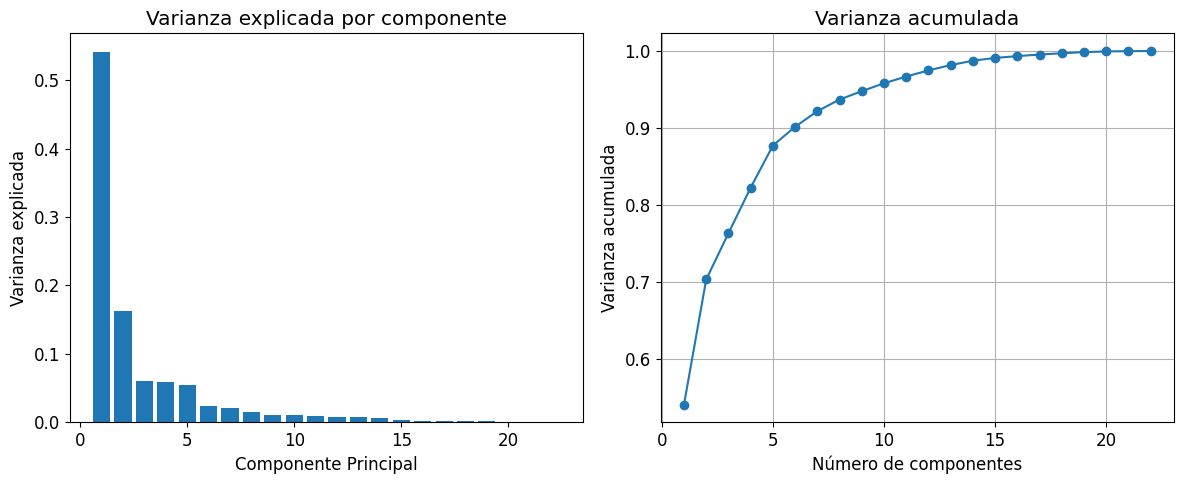
\includegraphics[width=0.48\textwidth]{images/varianza_acumulada.png}
    \caption{Gráfico de varianza acumulada y explicada por componente.}
    \label{fig:pca}
\end{figure}

\section{Determinación del Número Óptimo de Clusters}
El método del codo y el coeficiente de silueta indicaron que $k=2$ es una opción adecuada para separar los datos en grupos distintos.

\begin{figure}[htbp]
    \centering
    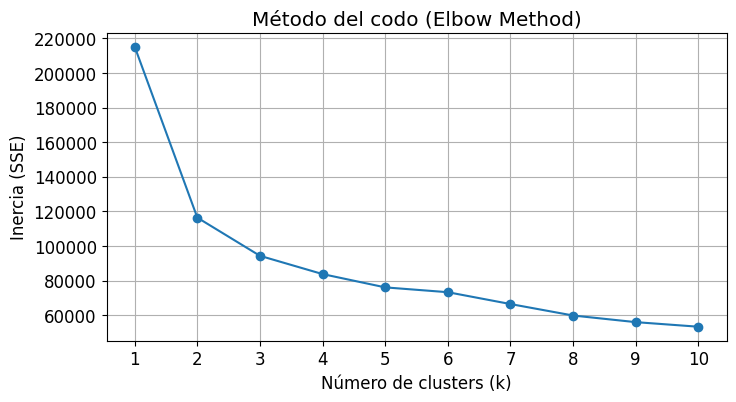
\includegraphics[width=0.48\textwidth]{images/elbow.png}
    \caption{Método del codo para determinar el número de clusters (k=2).}
    \label{fig:elbow}
\end{figure}

\begin{figure}[htbp]
    \centering
    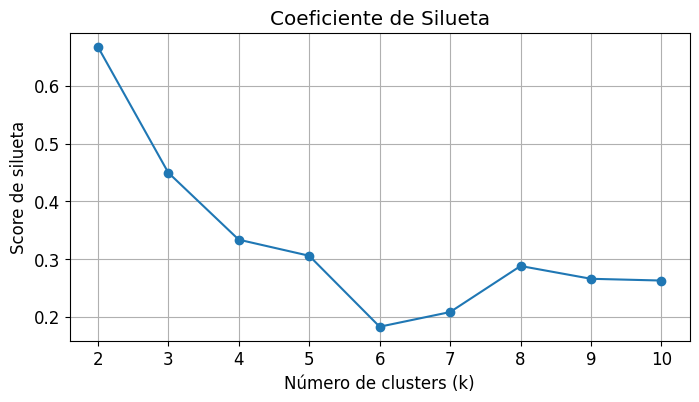
\includegraphics[width=0.48\textwidth]{images/silueta.png}
    \caption{Método de la silueta para determinar el número óptimo de clusters (k=2).}
    \label{fig:silueta}
\end{figure}

\section{Métodos de Clustering Aplicados}
Se aplicaron los siguientes algoritmos:

\begin{itemize}
    \item \textbf{K-Means:} produjo dos clusters bien separados pero muy polarizados.
        \begin{figure}[htbp]
            \centering
            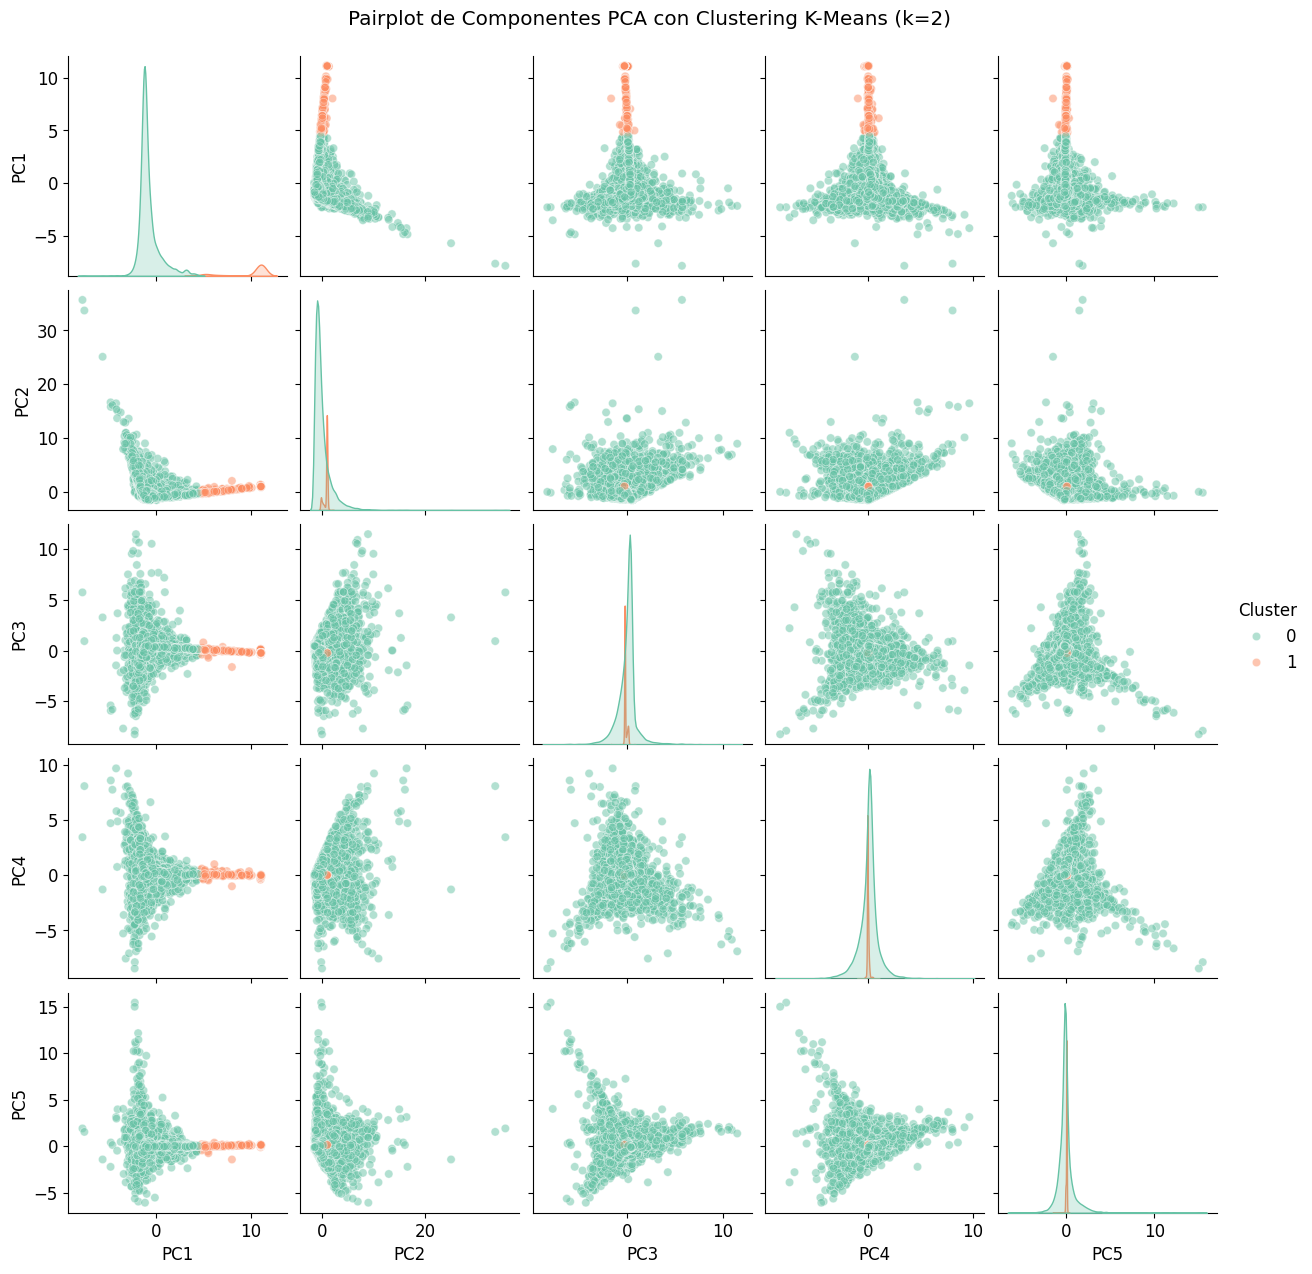
\includegraphics[width=0.48\textwidth]{images/k_means.png}
            \caption{Resultados de K-Means con k=2.}
            \label{fig:kmeans}
        \end{figure}
    \item \textbf{DBSCAN:} detectó ruido y grupos densos.
        \begin{figure}[htbp]
            \centering
            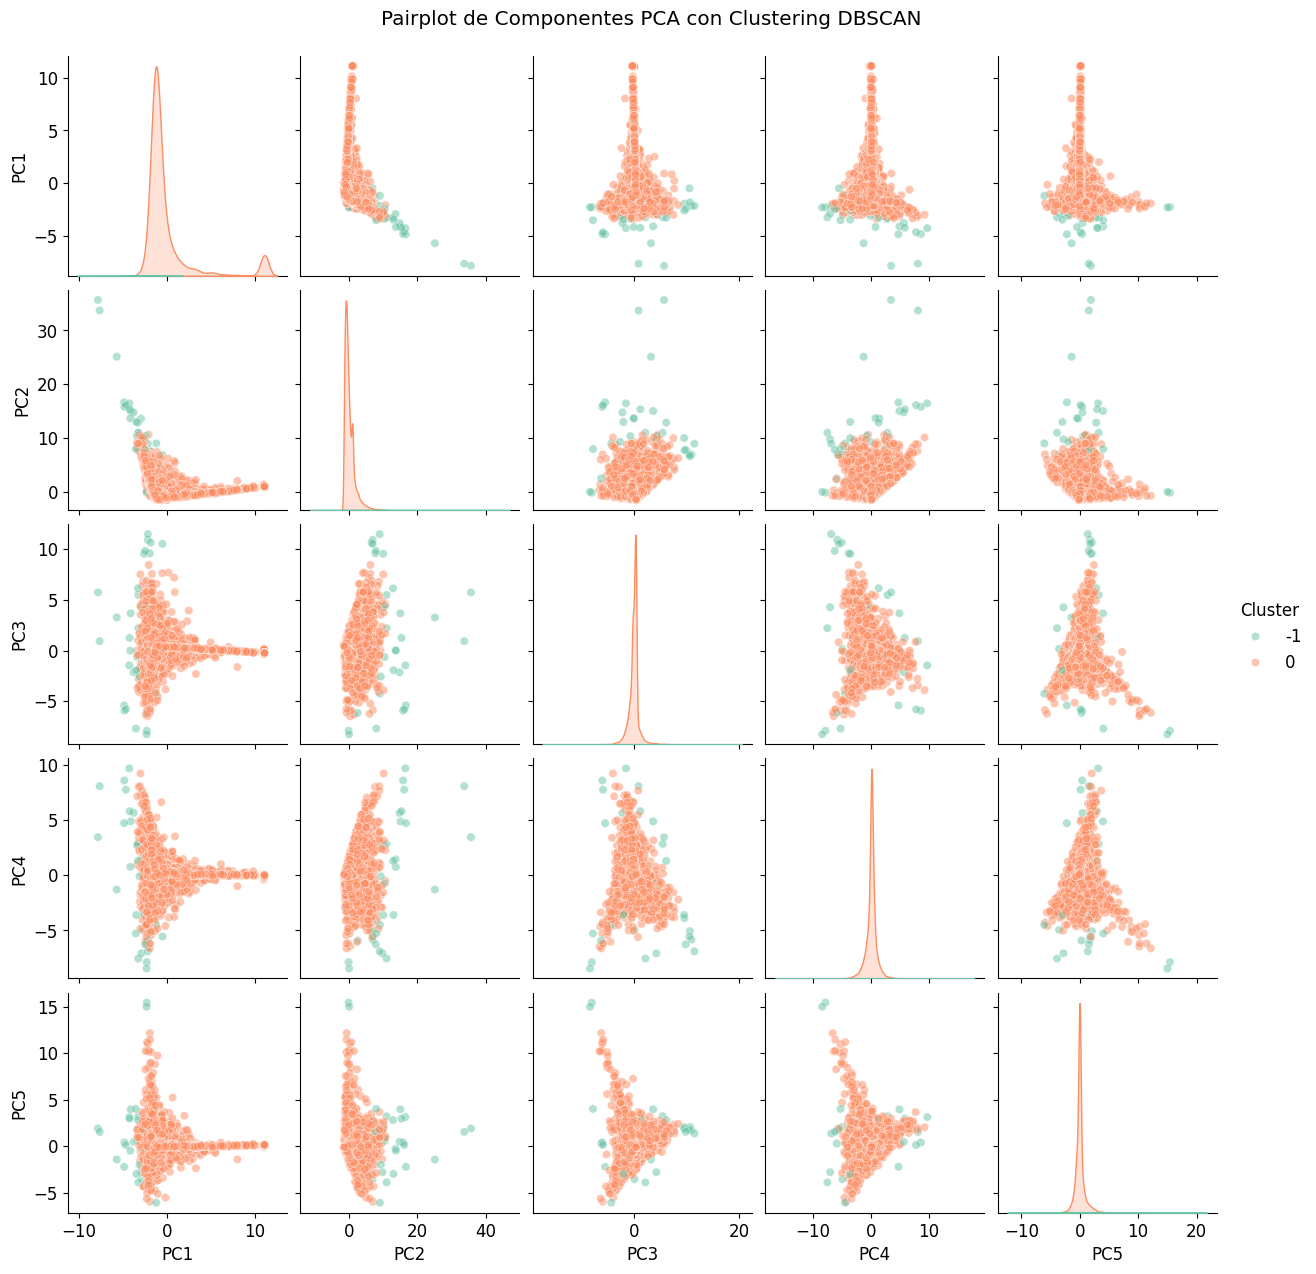
\includegraphics[width=0.48\textwidth]{images/dbscan.png}
            \caption{Resultados de DBSCAN.}
            \label{fig:dbscan}
        \end{figure}
    \item \textbf{Agglomerative Clustering:} identificó dos grupos similares a K-Means.
        \begin{figure}[htbp]
            \centering
            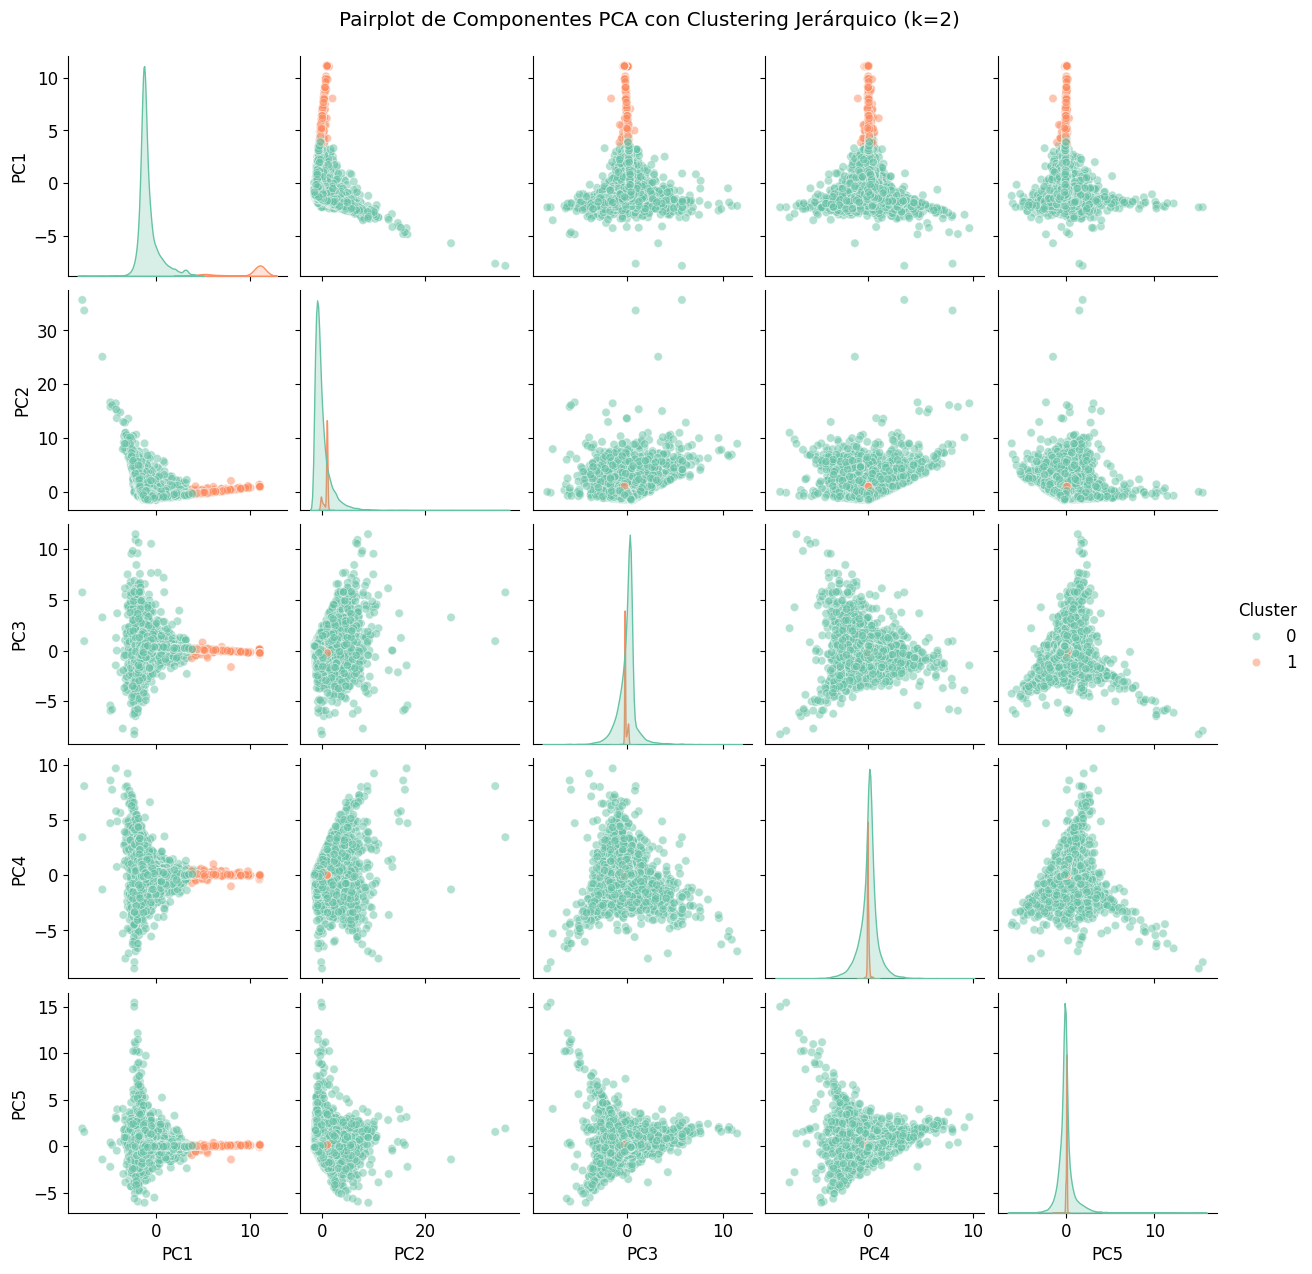
\includegraphics[width=0.48\textwidth]{images/jerarquico.png}
            \caption{Resultados de Agglomerative Clustering.}
            \label{fig:agglomerative}
        \end{figure}
    \item \textbf{Gaussian Mixture Models (GMM):} generó una segmentación probabilística, identificando también patrones en forma de núcleo y siendo mucho más flexible.
        \begin{figure}[htbp]
            \centering
            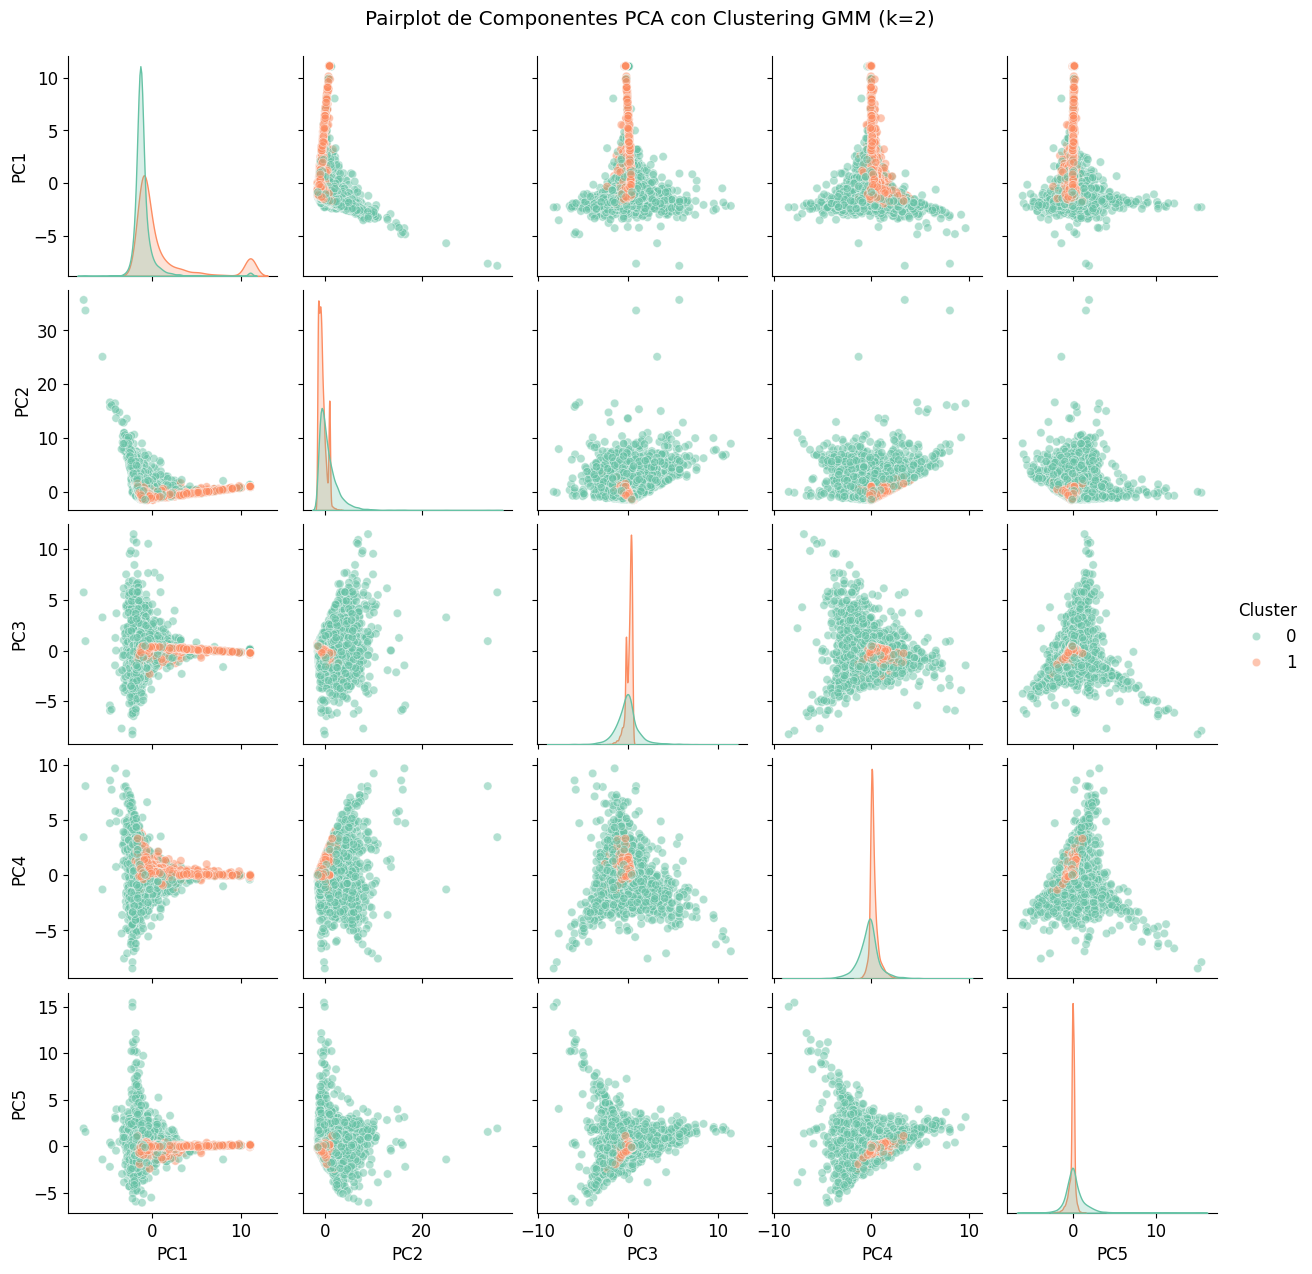
\includegraphics[width=0.48\textwidth]{images/gmm.png}
            \caption{Resultados de GMM.}
            \label{fig:gmm}
        \end{figure}
\end{itemize}

\section{Análisis de Resultados}
Los clusters encontrados se diferenciaron principalmente en las variables `BounceRates`,`ExitRates` y `SpecialDay`. Por lo que los resultados sugieren que un grupo corresponde a usuarios interesados y el otro a visitantes que abandonan rápidamente.

\section{Conclusiones}
El análisis permitió identificar dos perfiles principales de usuario. .

\begin{thebibliography}{99}
\bibitem{ref1} Sakar, C. O., et al. “Online Shoppers Purchasing Intention Dataset.” UCI Machine Learning Repository, 2018.
\bibitem{ref2} Han, J., Kamber, M., \& Pei, J. “Data Mining: Concepts and Techniques.” Morgan Kaufmann, 2011.
\end{thebibliography}

\end{document}
